\documentclass[10pt]{article}
\usepackage{pictex,amsmath,amsfonts,amssymb,amsthm,verbatim}
\usepackage{fullpage}
\usepackage{fullpage}
\usepackage{fancyhdr}
\usepackage{algorithm,algorithmic}
\usepackage{multirow}
\usepackage{gensymb}
\usepackage{mathrsfs}

\setlength{\voffset}{-0.25in}
\setlength{\headsep}{+0.5in}
\setlength{\parskip}{1em}
\setlength{\parindent}{0em}

\def\vu{\mathbf{u}}
\def\vv{\mathbf{v}}
\def\vb{\mathbf{b}}
\def\vw{\mathbf{w}}
\def\vs{\mathbf{s}}

%Font:
\usepackage{lmodern}
\renewcommand*\familydefault{\sfdefault} %% Only if the base font of the document is to be sans serif
\usepackage[T1]{fontenc}

%Graphics and stuff:
\usepackage{xcolor}
\usepackage{titlesec}
\usepackage{mdframed}
\usepackage{fancyhdr,fancybox}
\usepackage{lastpage}
\usepackage[utf8]{vietnam}\newmdenv[linecolor=blue,skipabove=\topsep,skipbelow=\topsep,leftmargin=5pt,rightmargin=-5pt,innerleftmargin=5pt,innerrightmargin=5pt]{mybox}

\pagestyle{fancy}
\fancyhead{}
\fancyfoot{} %clear all footer fields
\fancyfoot[L]{\scriptsize \ttfamily CC01 - Database System}
\fancyfoot[R]{\scriptsize \ttfamily Page {\thepage}/ \pageref{LastPage}}
\renewcommand{\headrulewidth}{0pt}
\renewcommand{\footrulewidth}{0.3pt}


%Macro:
\newcommand{\quotes}[1]{``#1''}
\newcommand{\tf}{\textbf}
\newcommand{\ti}{\textit}
\newcommand{\ttt}{\texttt}
\newcommand{\ud}{\underline}
\newcommand{\rarrow}{\rightarrow}
\newcommand{\larrow}{\leftarrow}
\newcommand{\lrarrow}{\leftrightarrow}


\usepackage{minted}
\usepackage{graphicx,graphics}

\begin{document}

\begin{center}
	\Huge DATABASE SYSTEM
\end{center}

%Table of contents:
\renewcommand*\contentsname{Contents:}
\tableofcontents

%Newpage
\newpage

\section{Chapter I: Introduction to Database}

\subsection{Some Definitions: }
\begin{itemize}
	\item Database is a collection of related data.
	\item Data is facts that can be recorded and have implicit meaning.
	\item Database Management System (DBMS) is a computerized system that enables users to create and maintain a database.
	\item DBMS is a \tf{general-purpose software system} that faciliates the processes of \ti{defining, constructing, manipulating} and \ti{sharing} databases among various users and applications.
\end{itemize}
	
\subsection{DBMS System:}
	\begin{itemize}
		\item \tf{Defining the database} involves specify the data types, structures, and constraints of the data to be stored in the database.
		\item \tf{Meta-data}, The database definition or descriptive information is also stored by the DBMS in the form of a database catalog and dictionary.
		\item \tf{Constructing the database} is the process of storing the data on some storage medium that is controlled by the DBMS.
		\item \tf{Manipulating the database} includes functions such as querying the database to retrieve specific data, updating the database to reflect changes in the miniworld.
		\item \tf{Sharing the database} allows multiple users and programs to access the database simultaneously.
	\end{itemize}

\subsection{Application Program:}
	\begin{itemize}
		\item An \tf{application program} accesses the database by sending queries or requests for data to DBMS.
		\item A \tf{query} typically causes data to be retrieved.
		\item A \tf{transaction} causes data to be read and written into the database.
	\end{itemize}

	- DBMS also provides functions for \tf{protecting} and \tf{maintaining} the database system:
	\begin{itemize}
		\item \tf{Protecting} includes \ti{system protection} against hardware or software malfuncton (or crash) and \ti{security protection} against unauthorized and malicious access. 
		\item A DBMS need to \tf{maintain} the database system by allowing the system as requirement change overtime.
	\end{itemize}

\bigbreak
\begin{mybox}
	\begin{center}
		Database system = database + DBMS
	\end{center}
\end{mybox}
	
	\bigbreak
	\begin{itemize}
		\item Conceptual Design.
		\item Logic Design.
		\item Physical Design.
	\end{itemize}

	- Design of the new application for an existing database or design of a brand new database starts off with a phase called \tf{requirements specification and analysis}. \\

	- These requirements are documented in detail and transformed into a \tf{conceptual design} that can be represented and manipulated by some computerized tools $\rightarrow$ easily modified, maintained and transformed into \tf{database implementation}. \\

	- The design is then translated into \tf{logical design}. that can be expressed in a data model implemented in a commercial DBMS. \\

	- The final stage is called \tf{physical design}, further specifications are provided for storing and access database. \\

\subsection{Characteristic of the Database Approach: }
\begin{enumerate}
	\item File processing:
	\begin{itemize}
		\item A traditional \tf{file processing}, each user defines and implements the files needed for the specific software application.
		\item Both users are interested in same data but each users maintain separate files and programs to manipulate files.
		\item This redundancy in defining and storing data results in wasted storage space and in redundant effort to maintain common up-to-date data.
	\end{itemize}

	\item Database Approach:
	\begin{itemize}
		\item In database approach, a single repository maintains data that defined once and then accessed by various users repeatedly though queries, transactions, and application programs.
		\item The main characteristic of the database approach vs file processing:
		\begin{itemize}
			\item Self-describing nature of a database system.
			\item Insulation (ngăn cách) between programs and data, and data abstraction.
			\item Support of the multiple views of the data.
			\item Sharing of data and multi-user transaction processing.
		\end{itemize}
	\end{itemize}

	\begin{enumerate}
		\item Self-Describing Nature of a Database System:
		\begin{itemize}
			\item The database system contain not only the database itself but also a complete definition or description of database structure and constraints.
			\item The information stored in the DBMS catalog is called \tf{meta-data}, it describes the structure of the primary database.
			\item NOSQL systems do not require meta-data, those data is stored in \tf{self-describing data} that includes the data item names and data values together in 1 structure.
			\item The DBMS software must work equally well with \ti{any number of database applications}
		\end{itemize}

		\item Insulation between Programs and Data, and Data Abstraction:
		\begin{itemize}
			\item The structure of data files is stored in the DBMS catalog separately from the access program, this is called \tf{program-data independence}. \\
			(Why \tf{meta-data enable data-program independence ?})
			\item An operation (known as function or method) is specific in \ti{interface} and \ti{implementation}.

			\begin{itemize}
				\item interface includes operation name and its data types of its argument.
				\item implementation of the operation is specified separately and can be changed without affecting the interface.
			\end{itemize}

			\item This may be known as \tf{program-operation independence}.
			\item The characteristic that allows program-data independence and program-operation independence is called \tf{data abstraction}.
			\item A \tf{data model} is a type of data abstraction that is used to provided this conceptual representation. The data model \ti{hides} storage and implementation out of database users.  
		\end{itemize}

		\item Support of multiple views of the Data: 
		\begin{itemize}
			\item A multi-user DBMS whose users have a variety of distinct applications must provide facilities for multiple views.
		\end{itemize}

		\item Sharing of Data and Multi-user Transaction Processing: 
		\begin{itemize}
			\item This is essential if data for multiple users to be integrated and maintained for a single database.
			\item The DBMS must include \tf{concurrency control} software to ensure that several users trying to update the same data so that the results of update is correct.
		\end{itemize} 
	\end{enumerate}

	\item Actors on the Scene:
	\begin{itemize}
		\item Database Administrators.
		\item Database Designers.
		\item End users.
	\end{itemize}
\end{enumerate}

\subsection{Advantages of Using the DBMS Approach}
\begin{enumerate}
	\item Reduce Redundancy:
	\begin{itemize}
		\item Data normalization: All logical data item are stored in \ti{only one place} in the database.
	\end{itemize} 

	\item Restricting Unauthorized Access:
	\item Provide persistent storage for Program Object:
	\item Provide Storage Structures and Search Techniques for efficient Query processing:
	\item Provide Backup and Recovery:
	\item Provide Multiple User Interfaces:
	\item Represent Complex Relationships among Data:
	\item Enforcing Integrity Constraints:
	\item Permitting Interfencing and Actions using Rules and Triggers:
\end{enumerate}

\subsection{When not to use DBMS}
\begin{enumerate}
	\item It maybe more desirable to develop customized database applications:
	\begin{itemize}
		\item Simple, well-defined database applications that are not expected to change at all.
		\item Stringent, real-time requirements for some application programs that may not met base of DBMS overhead.
		\item Embedded devices with limited storage capacity, where a general-purpose DBMS would not fit.
		\item No multiple user-access data.
	\end{itemize}
\end{enumerate}

\bigbreak
\section{Chapter II: Database System Concepts and Architecture}

\subsection{Data Models, Schemas, and Instances}
\begin{enumerate}
	\item Data Models:
	\begin{itemize}
		\item A data model is a collection of concepts that can be used to describe the structure of the database - provides the necessary means to achieve this abstraction.
		\item Most data models also include set of \tf{basic operations} for specifying retrievals and updates on the database.
		\item Types of Data Model:
		\begin{itemize}
			\item \tf{High-level} or \tf{conceptual data models} provide concepts that are close to the way many users realize data.
			\item \tf{Low-level} or \tf{physical data model} provide concepts that describe the detail of how data is stored in the computer storage media, typically magnetic disk.
			\item \tf{Representational} (or \tf{implementation}) \tf{data models} provide concepts that may be easily understood by end users but that are not \underline{too far removed} (very different from) from the way data is organized in computer storage.
		\end{itemize}
	\end{itemize}

	\item Schemas, Instances, and Database State:
	\begin{itemize}
		\item Schemas is kind of layout of the database.
		\item The actual data in the database may change quite frequently. The data in the database at the particular moment of time is called a \tf{database state} or \tf{snapshot}
	\end{itemize}
\end{enumerate}

\subsection{Three-Schema Architecture and Data Independence}
\begin{enumerate}
	\item The three-schema Architecture: \\
	
	%\includegraphics[scale = 0.5]{hinh.png}

	\begin{itemize}
		\item The \tf{internal level} has an \tf{internal schema} describes the physical storage structure of the database.
		\item The \tf{conceptual level} has a \tf{conceptual schema} describes the structure of the whole database for users.
		\item The \tf{external} or \tf{view level} includes a number of \tf{external schemas} or \tf{user views}.
	\end{itemize}

	\item Data Independence: 
	\begin{enumerate}
		\item \tf{Logical data independence:} is the capacity to change the conceptual schema without having to change external schemas or application programs.
		\item \tf{Physical data independence:} is the capacity to change the internal schema without having to change the conceptual schema
		\item Summary: Data independence occurs when the schema is changed at some level, the schema at the next higher level remains unchanged; only the \ti{mapping} between the two levels is changed. Hence, plication referring to the higher level schema do not need to be changed.

		\bigbreak
		%\includegraphics[scale = 0.5]{hinh1.png}
		\bigbreak 
	\end{enumerate}
\end{enumerate}

\subsection{Database Languages and Interfaces}
\begin{enumerate}
	\item DBMS Languages:
	\begin{itemize}
		\item \tf{Data definition language} (DDL) : used to define both conceptual and external schemas where no strict separation of levels is maintained.
		\item \tf{Storage definition language} (SDL):
		\begin{itemize}
			\item is used to specify the internal schema.
			\item DDL is used in conceptual schema.
			\item It is used where there is a clear separation between the conceptual and external levels
		\end{itemize}  
		\item \tf{View definition language} (VDL) : is used to specify user views and their mapping to the conceptual and external schemas.
		\item Beside, DBMS also provides a set of operations or a language called the \tf{data manipulation language} (DML) for manipulating the database. \\

		\begin{itemize}
			\item A \tf{high-level} or \tf{nonprocedural} DML.
			\begin{itemize}
				\item It is used to specify complex database operations concisely (chính xác).
				\item Many DBMSs allow high-level DML statements to be entered from the display monitor or terminal or to be embedded in a general-purpose programming language.
				\item High-level DML, such as SQL can specify and retrieve many records in a single DML statement, it is called \tf{set-at-a-time} 
			\end{itemize}
			\item A \tf{low-level} or \tf{procedural} DML.
			\begin{itemize}
				\item It \ti{must} be embedded in a general-purposes language.
				\item It is also called as \tf{record-at-a-time} since it functions related to retrieving and processing individuals records and objects.
			\end{itemize}
		\end{itemize}

		\item Whenever DMLS commands, whether high-level or low-level, are embedded in a general-purpose language and that language is called the \tf{host language} and DML is called the \tf{data sub language}.
		\item A high-level DML used in a standalone interactive manner is called a \tf{query language}.
	\end{itemize}

	\item DBMS Interfaces:
	\begin{itemize}
		\item Menu-based Interfaces for Web Clients or Browsing
		\item Apps for Mobile Devices
		\item Forms-based Interfaces
		\item Graphic User Interfaces
		\item Natural Language Interfaces
		\item Keyboard-based Database Search
		\item Search Input and Output
	\end{itemize}
\end{enumerate}

\subsection{The Database System Environment}
\begin{enumerate}
	\item \tf{DBMS Component Modules}
	\begin{itemize}
		\item Many DBMSs have \tf{buffer management} module to schedule disk read/write since management of buffer storage has a considerable effect on performance by reducing disk read/write.
		\item A high-level \tf{sorted data manager} module of the DBMS controls access to DBMS information that is stored on disk, whether it is part of the database or the catalog.
	\end{itemize}

	\item \tf{Database System Utilities}
	\begin{itemize}
		\item Most DBMSs have \tf{database utilities} to help the DBA manage the database system.
		\begin{itemize}
			\item Loading
			\item Backup
			\item Database storage reorganization
			\item Performance monitoring (monitors database and provide video statistics to the DBA)
		\end{itemize} 
	\end{itemize}
\end{enumerate}

\bigbreak
\begin{center}
	End
\end{center}
\pagebreak

\section{Chapter III: Conceptual Data Modeling and Database Design}

\quotes{The conceptual schema is a concise description of the data requirements of the users and includes detailed descriptions of the entity types, relationships, and constraints, using the concept provided by high-level data model.}

\quotes{ER model is a logical organization of data within a database system. ER model technique is based on relational data model}

\subsection{Entity Types, Entity Sets, Attributes, and Keys}
\begin{enumerate}
	\item \tf{Entity}
	\begin{itemize}
		\item Entity is a \ti{thing} or \ti{object} in the real world with an independence existence.
		\item An entity may be an object with a physical existence or it may be an object with a conceptual existence (Ex: company, university jobs, etc).
	\end{itemize}

	\item \tf{Attribute}
	\begin{itemize}
		\item Each entity has attributes - the particular properties that describe it.
		\item Types of attributes in the ER model:
		\begin{itemize}
			\item \tf{Composite versus Simple}
			\begin{itemize}
				\item \tf{Composite attributes} can be divided into smaller subparts, which represent more \tf{basic} attributes with independence meanings.
				\item Attributes that are not divisible are called \tf{simple} or \tf{atomic attributes} 
			\end{itemize}

			\item \tf{Single-Valued versus Multivalued Attributes}
			\begin{itemize}
				\item Attributes have a single value for a particular entity are called \tf{single valued entity}.
				\item Attributes have a multiple value for a particular entity are called \tf{multivalued entity}.
			\end{itemize}

			\item \tf{Stored versus Derived Attributes}
			\begin{itemize}
				\item Attributes that are related to or can be determined by another attributes are called \tf{derived attributes}.
				\item The others are called \tf{stored attributes}.
			\end{itemize}

			\item \tf{NULL Values}
			\begin{itemize}
				\item Attributes that particular entities may not have an applicable value for. (\ti{not applicable})
				\item NULL can be also be used if we do not know the value of an attribute for a particular entity. (\ti{unknown}) 
			\end{itemize}

			\item \tf{Complex Attributes}: composite and multivalued can be nested arbitrarily.
		\end{itemize}
	\end{itemize}
	\item \tf{Entity Types and Entity Sets}
	\begin{itemize}
		\item An \tf{entity type} defines a \ti{collection} (or \ti{set}) of entities that have the same attributes.
		\item Each entity type in the database is described by its name and attributes.
		\item The collection of all entities of a particular entity type in the database at any point is called an \tf{entity set} or \tf{entity collection}.
		\item The entity set is usually referred to using the same name as the entity type, even though they are two separate concepts.
		\item An entity type describes the \tf{schema} or \tf{intension} for \ti{a set of entities} that share the same structure.
		\item The collection of entities of a particular entity type is grouped into an entity set, which is also called the \tf{extension} of the entity type.
	\end{itemize}

	\item \tf{Key Attributes of an Entity Type}
	\begin{itemize}
		\item An important constraint on the entities of an entity type is the \tf{key} or \tf{uniqueness constraint} on attributes.
		\item An entity type has one or more attributes whose values are distinct for each individual entity in the entity set, those attributes are called \tf{key attributes}, and its value can be used to identify each entity uniquely.
		\item An attribute is a key of an entity type means that the preceding uniqueness property must hold for \ti{every entity set} of the entity type.   
	\end{itemize}

	\item \tf{Value Sets (Domains) of Attributes}
	\begin{itemize}
		\item Each simple attribute of an entity type is associated with a \tf{value set} (or \tf{domain} of the values), which specifies the set of values that may be assigned to that attribute for each individual entity. 
	\end{itemize}	
\end{enumerate}

\subsection{Relationship Types, Relationship Sets, Roles, and Structural Constraints}
\begin{enumerate}
	\item Relationship Types, Sets, and Instances
	\begin{itemize}
		\item \tf{Relationship Types, Sets, and Instances}
		\begin{itemize}
			\item A \tf{relationship type} R among n entity types $E_{1}, E{2}, \ldots, E_{n}$ defines a set of associations - or a \tf{relationship set} - among entities from these entity types.
			\item The relationship set R is a set of \tf{relationship instances} $r_{i}$, where each $r_{i}$ associates n individual entities ($e_{1}, e_{2}, \ldots, e_{n}$) and each entity $e_{j}$ in $r_i$ is a member of entity set $E_{j}$.
		\end{itemize}

		\item \tf{Relationship Degree, Role Names, and Recursive Relationships}
		\begin{itemize}
			\item \tf{Degree of a Relationship Type}
			\begin{itemize}
				\item The \tf{degree} of a relationship type is the number of participating entity type.
			\end{itemize}

			\item \tf{Relationship as Attributes}
			\item \tf{Role Names and Recursive Relationships}
			\begin{itemize}
				\item The \tf{role name} signifies the role that a participating entity from the entity type plays in each role relationship instance, and it helps to explain what the relationship means.
				\item Role name are not technically necessary in relationship types where all the participating entity are distinct, since each participating entity type name can by used as the role name.
				\item In case the \ti{same} entity type participates in a relationship type in \ti{different roles}, the role name becomes essential. \\
				$\rightarrow$ Such relationship types are called \tf{recursive relationship} or \tf{self-referencing relationships}. 
			\end{itemize}
		\end{itemize}

		\item \tf{(Structural) Constraints on Binary Relationships Types}
		\begin{itemize}
			\item \tf{Cardinality Ratios for Binary Relationships}
			\begin{itemize}
				\item The \tf{cardinality ratio} for a binary relationship specifies the \ti{maximum} number of relationship instances that an entity can participate on.
			\end{itemize}

			\item \tf{Participation Constraints and Existence Dependencies}
			\begin{itemize}
				\item The \tf{participation constraint} specifies whether the existence of an entity depends on its being related to another entity via the relationship type.
				\item This constraint specifies the \ti{minimum} number of relationship instances that each entity can participate in, called the \tf{minimum cardinality constraint}.
				\item There are two types of participation constraints:
				\begin{itemize}
					\item \tf{Total participation: } every entity in the total set of entities must related to another entity set via a relationship, called \tf{existence dependency}
					\item \tf{Partial Participation: } some or \ti{some or part of the set of} entities are related to some other entities via a relationship. 
				\end{itemize}
			\end{itemize}
		\end{itemize}

		\item \tf{Attributes of Relationship Types}
		\begin{itemize}
			\item Relationship types can also have attributes, similar to those of entity types.
			\item The attributes of 1:1 relationship types can be determined separately, as either one of the participating types.
			\item However, for 1:N relationship types, a relationship attribute can be migrated \ti{only} to the entity type on the N-side of the relationship.
			\item For M:N (many-to-many) relationship types, some attributes may be determined by the \ti{combination of participating entities} in a relationship instance, not by any single entity. Such attributes must be \ti{specified as relationship attributes}.
		\end{itemize}
	\end{itemize}
\end{enumerate}

\subsection{Weak Entity Types}
\begin{enumerate}
	\item \tf{Definitions: }
	\begin{itemize}
		\item Entity types that do not have key attributes of their own are called \tf{weak entity types}.
		\item In contrast, \tf{regular entity types} that do have a key attributes are called \tf{strong entity types}.
		\item Entities belonging to a weak entity type are identified by being related to specific entities from another entity type in combination with one of their attribute values. Those entities are called \tf{identifying} or \tf{owner entity type}.
		\item Relationship type that relates to a weak entity type to its owner is called \tf{identifying relationship} of the weak entity type.
		\item A weak entity type always have a \ti{total participation constraint} (existence dependency) with respect to its identifying relationship because a weak entity cannot be identified without an owner entity.
		\item A weak entity type normally has a \tf{partial key}. which is the attribute that can uniquely identify weak entities that are related to the \ti{same owner entity}. In a worst case, a composite attribute of \ti{all the weak entity's attributes} will be the partial key.
		\item Weak entity types can sometimes be represented as complex (composite, multivalued) attributes.
	\end{itemize}
\end{enumerate}

\subsection{Proper Naming of Schema Constructs}
\begin{itemize}
	\item \ti{Singular Names} are chosen to named for entity types, rather than plural names because the entity type name applies to each individual entity belonging to that entity type.
	\item Entity type and relationship type names are in uppercase letters, attribute names have their initial letter capitalized, and role names are in lowercase letters. 
\end{itemize}

\subsection{Notation for ER Diagrams}
%\includegraphics[scale = 0.4]{hinh2.png}
\bigbreak

\subsection{Other Notation: UML Class Diagrams}

\subsection{Relationship Types of Degree Higher than Two}
\bigbreak

\subsection{Choosing between Binary and Ternary (or Higher-Degree) Relationships}
\bigbreak

\subsection{Constraints on Ternary (or Higher-Degree) Relationships}
\bigbreak

\subsection{Another Example: A UNIVERSITY Database}
\bigbreak

\begin{center}
	End
\end{center}
\pagebreak

%----------------------------------------------------------------%
\section{Chapter IV: The Enhanced Entity - Relationship (EER) Model}

\subsection{Subclasses, Superclasses, and Inheritance}

\quotes{The EER model includes \ti{all} the \ti{modeling concepts of the ER model}. In addition, it includes the concepts of \tf{subclass} and \tf{superclass} and the related concepts of \tf{specialization} and \tf{generalization}.}

\begin{enumerate}
	\item \tf{Subclass:} A set of subset of the entities that belong to the entity set. Subclasses can also have \tf{specific} (or local) \ti{attributes} and \tf{relationships}.
	\item \tf{Superclass:} An entity set of subclasses.
	\item An entity cannot exist in the database merely by being a member of a subclass, it must also be a member of the superclass, an entity can be also included as a member of any number of subclasses.
	\item \tf{Inheritance: }
	\begin{itemize}
		\item An entity in the subclass represents the same real-world entity from the superclass, it should process values for its specific attributes \ti{as well as} values of its attributes as a member of the superclass.
	\end{itemize}
	$\rightarrow$ The subclass \tf{inherits} all the attributes of the entity as a member of the superclass. \\
	$\rightarrow$ The entity also \tf{inherits} all the relationships in which the superclass participates.
\end{enumerate}

\subsection{Specialization and Generalization}
\begin{enumerate}
	\item \tf{Specialization: }
	\begin{itemize}
		\item \tf{Specialization:} is the process of defining \ti{a set of subclasses} of an entity type; this entity type is called the \ti{superclass} of specialization.
		\item There are two main reasons for including class/subclass relationships and specializations:
		\begin{itemize}
			\item The first:
			\begin{itemize}
				\item Certain attributes may apply to some but not all entities of the superclass entity type.
				\item A subclass is defined in order to group the entities to which these attributes apply.
				\item The members of the subclass may still share the majority of their attributes with the other members of the superclass.
			\end{itemize}

			\item The second:
			\begin{itemize}
				\item Some relationship types may be participated in only by entities that are members of the subclass.  
			\end{itemize}
		\end{itemize}
	\end{itemize}

	\item \tf{Generalization}
	\begin{itemize}
		\item A \ti{reverse process} of abstraction in which we suppress the differences among the several entity types, identify their common features, and \tf{generalize} them into a single \tf{superclass}.
		\item the Generalization process can be viewed as being functionally the inverse of the specialization process.
	\end{itemize}
\end{enumerate}

\subsection{Constraints and Characteristics of Specialization and Generalization Hierarchies}

\begin{enumerate}
	\item \tf{Constraints on Specialization and Generalization}
	\begin{itemize}
		\item In some specializations we can determine exactly the entities that will become members of each subclass by placing a condition on the value of some attribute of the superclass. Such classes are called \tf{predicate-defined} (or \tf{condition-defined}) subclasses.
		\item If \ti{all} subclasses in a specialization have their membership condition on the \ti{same} attribute of the superclass, the specialization itself is called an \tf{attribute-defined specialization}, and the attribute is called \tf{defining attribute} of the specialization.
		\item When we do not have a condition for determining membership in a subclass, the subclass is called \tf{user-defined}.
		\item \tf{Disjointness constraint: } 
		\begin{itemize}
			\item It specify that the subclass of the specialization must be disjoint sets.
			\item This means that an entity can be a member of at \ti{most} one of the subclasses of the specialization.
			\item A specialization that is attribute-defined implies the disjointness constraints. (if the attribute used to define the membership predicate is single-valued).
			\item The \tf{d} in the circle stands for \ti{disjoint}, the \tf{d} notation also applies to user-defined subclasses of a specialization that must be disjoint. 
		\end{itemize}
		\item \tf{Overlapping constraint: } 
		\begin{itemize}
			\item the same(real-world) entity may be a member of more than one subclass of the specialization.
			\item The \tf{o} notation is used to present overlapping.
		\end{itemize}

		\item \tf{Completeness} (or \tf{totalness} constraint):
		\begin{itemize}
			\item A \tf{total specialization} constraint specifies that \ti{every entity} in the superclass must be a member of at least one subclass in the specialization.
			\item A \tf{partial specialization} constraint allows an entity not to belong to any of the subclasses.
			\item The disjointness and completeness constraints are \ti{independent}:
			\begin{itemize}
				\item Disjoint, total
				\item Disjoint, partial
				\item Overlapping, total
				\item Overlapping, partial
			\end{itemize}

			\item A superclass that was identified through the \ti{generalization} process usually is \tf{total}, because the superclass is \ti{derived from} the subclasses and hence only the entities that are in the subclasses.
		\end{itemize}

		\item For insertion and deletion rules to specialization (and generalization) as a consequence of the constraints should follow the rules:
		\begin{itemize}
			\item Deleting an entity from a superclass implies that it is automatically deleted from all the subclasses to which it belongs.
			\item Inserting an entity in a superclass implies that the entity is \tf{mandatorily} inserted in all \ti{predicate-defined} (or attribute defined) subclasses for which the entity satisfies the defining predicate.
			\item Inserting an entity in a superclass of a \ti{total specialization} implies that the entity is madatorily inserted in at least one of the subclasses of the specialization
		\end{itemize}
	\end{itemize}
\end{enumerate}

\subsection{Specialization and Generalization Hierarchies and Lattices}
\begin{itemize}
	\item A subclass itself may have further subclasses specified on it, forming a hierarchy or a lattice of specialization.
	\item A \tf{specialization hierarchy} has the constraint that every subclass participate \tf{as a subclass} in \ti{only one class/subclass} relationship $\rightarrow$ Each subclass has only one parent, which \tf{result} in a \tf{tree structure} or \tf{strict hierarchy}.
	\item For a \tf{specialization lattice}, a subclass can be a subclass in \ti{in more than} class/subclass relationship.
	\item A subclass inherits the attributes not only of its direct superclass, but also of all its predecessor subclasses \ti{all the way to the root} of the hierarchy or lattice if necessary.
	\item A \tf{leaf node} is a class that has \ti{no subclasses of its own}.
	\item A subclass with \ti{no more than one} superclass is called a \tf{shared subclass} $\rightarrow$ This lead to the concept known as \tf{multiple inheritance}
	\item The existence of at least one shared subclass leads to a lattice (and hence to \ti{multiple inheritance}); if no shared subclasses existed, we would have a hierarchy rather than a lattice and only \tf{single inheritance} would exist.
	\item If an attribute (or relationship) originating in the \ti{same superclass} is inherited more than once via different paths in the lattice, then it should be included only once in the shared subclass.   
\end{itemize}

\subsection{Utilizing Specialization and Generalization in Refining Conceptual Schemas}
\begin{itemize}
	\item \tf{top-down conceptual refinement} or \tf{bottom-up conceptual refinement}
\end{itemize}

\subsection{Modeling of UNION Types Using Categories}

\quotes{A subclass represent a collection of entities that is a subset of the UNION of entities from distinct entity types, that subclass is called a \tf{union type} or \tf{category}}

\begin{enumerate}
	\item A category has two or more superclass that may represent collections of entities from \ti{distinct entity types}, whereas other superclass/subclass relationships always have a single superclass.
	\item (Read textbook) Differences between a lattice and a category.
	\item (Read textbook) Difference between a generalization and a category.
	\item A category can be \tf{total} or \tf{partial}:
	\begin{itemize}
		\item A total category holds the \ti{union} of all entities in its superclass.
		\item A partial category can hold the \ti{subset of the union}.
	\end{itemize}
\end{enumerate}

\begin{center}
	End
\end{center}
\pagebreak

%------------------------------------------------------------------%

\section{Chapter 5: The Relational Data Model and Relational Database Constraints}

\begin{itemize}
	\item The relational model was first introduced by Ted Codd of IBM Research in 1970 in a classic paper.
	\item The model uses the concept of a \ti{mathematical relation} - which looks somewhat like a table of values.
	\item The first commercial implementations of the relational model became available in the early 1980s, such as the SQL/DS system on the MVS operating system by IBM and the Oracle DBMS. 
\end{itemize}

\subsection{Relational Model Concepts}

\begin{itemize}
	\item The relational model represents the database as a collection of \ti{relations}.
	\item When a relation is thought of as a \tf{table} of values, each row in the table represents a collection of related data values.
	\begin{itemize}
		\item A row represents a fact that typically corresponds to a real-world entity or relationship.
		\item The table name and column names are used to help to interpret the meaning of the values in each row.
	\end{itemize}
	\item in the formal relational model terminology, a row is called \ti{tuple}, a column header is called an \ti{attribute}, and the table is called a\ti{relation}.
	\item The data type describing the types of values that can appear in each column is represented by a \ti{domain} of possible values.
\end{itemize}  

\begin{enumerate}
	\item \tf{Domains, Attributes, Tuples, and Relations}
	\begin{itemize}
		\item A \tf{domain} D is set of atomic values. By \tf{atomic} we mean that each value in the domain is indivisible as far as the formal relational model is concerned.
		\item A domain is given a name, data type, and format.
		\item A \tf{relational schema} R, denoted by $R(A_1, A_2, \ldots, A_n)$, is made up of a relation name R and a list of attributes, $A_1, A_2, \ldots, A_n$.
		\begin{itemize}
			\item Each \tf{attribute} $A_i$ is the name of a role played by some domain D in the relation schema R.
			\item D is called the \tf{domain} of $A_{i}$ and is denoted by \tf{dom($A_i$)}.
			\item A relation schema is used to \ti{describe} a relation; R is called the \tf{name} of this relation.
			\item The \tf{degree} (or \tf{arity}) of a relation is the number of attributes n of its relation schema.
		\end{itemize}
		\item For example, A relation of degree seven, which store information about university students, would contain seven attributes describing each student as follow: \\
		\begin{center}
		STUDENT(Name, Ssn,\ttt{Home\_phone}, Address, \ttt{Office\_phone}, Age, Gpa)
		\end{center}
		\item Using data type of each attribute, the definition is sometimes written as:
		\begin{center}
		STUDENT(Name: string, Ssn: string, \ttt{Home\_phone}: string, Address: string, \ttt{Office\_phone}: string, Age: integer, Gpa: real)
		\end{center}

		\item We can specify the domain for STUDENT: dom(Gpa) = \ttt{Grade\_point\_averages}.
		\item A \tf{relation} (or \tf{relation state}) \ti{r} of the relation schema R$(A_1, A_2, \ldots, A_n)$ also denoted by r(R), is a set of n-tuples r = ${t_1, t_2, \ldots, t_m}$.
		\item Each n-\tf{tuple} t is an ordered list of n values t $=<v_1, v_2, \ldots, v_n>$, where each value $v_i$, $1 \le i \ge n$, is an element of dom($A_{i}$) or is a special NULL value.
		\item The \ti{i}th value in tuple t, which corresponds to the attribute $A_{i}$, is referred to as t$[A_{i}]$ or t.$A_{i}$ (or \ti{t[i]} if we use the positional notation).
		\item A \tf{relation intension} is used for schema R and the term \tf{relation extension} is used for a relation state r(R).
		\item \tf{Cardinality} is the number of \ti{tuples} in the table.
		\item It is possible for several attributes to \ti{have the same domain}. The attribute names indicate different \tf{roles}, or interpretations, for the domain.
	\end{itemize}

	\item \tf{Characteristic of Relations}
	\begin{itemize}
		\item \tf{Ordering of Tuples in a Relation: }
		\begin{itemize}
			\item A relation is defined as a \ti{set of tuples}; elements of a set have \ti{no order} among them; hence tuples in a relation do not have any particular order.
			\item A relation is not sensitive to the ordering of tuples. When we display a relation as a table, the rows are displayed in a certain order. 
		\end{itemize}

		\item \tf{Ordering of Values within Tuple and an Alternative Definition of a Relation: }
		\begin{itemize}
			\item An \tf{alternative definition} of a relation can be given, making the ordering of values in a tuple unnecessary. In this definition, a relation schema R = ${A_1, A_2,\ldots, A_n}$ is a set of attributes (instead of an ordered list of attributes), and a relation state r(R) is a finite set of mappings r = ${t_1, t_2,\ldots, t_m}$, where each tuple ti is a mapping from R to D, and D is the union (denoted by $\cup$) of the attribute domains; that is, $D = dom(A_1) \cup dom(A_2) \cup \ldots \cup dom(A_n)$. In this definition, $t[A_i]$ must be in $dom(A_i)$ for $1 \le i \le n$ for each mapping t in r. Each mapping $t_i$ is called a tuple.
			\item According to this definition of tuple as a mapping, a tuple can be considered as a set of (<attribute>, <value>) pairs, where each pair gives the value of the mapping from an attribute $A_i$ to a value $v_i$ from $dom(A_i)$.
			\item The ordering of attributes is not important, because the attribute name appears with its value.
			\item When the attribute name and value are included together in a tuple, it is known as \tf{self-describing data}, because the description of each value (attribute name. is included in the tuple.
		\end{itemize}

		\item \tf{Values and NULLs in the Tuples: }
		\begin{itemize}
			\item Each value in a tuple is an \tf{atomic} value.
			\item Composite and multivalued attributes are not allowed. In relational model, multivalued attributes must be represented by separate relations, and composite attributes are represented only by their simple component attributes.
			\item \tf{flat relational model}, must of theory behind the relational model was developed with this assumption in mind, which is called \tf{first normal form} assumption.
			\item In general, we can have several meanings for NULL values, such as \tf{value unknown, value} exists but is \tf{no available}, or \tf{attribute does not apply} to this tuple (also known as \tf{value undefined}).
		\end{itemize}

		\item \tf{Interpretation (Meaning) of a Relation}
		\begin{itemize}
			\item The relation schema can be interpreted as a declaration or a type of \tf{assertion}.
			\item Each tuple in the relation can then be interpreted as a \tf{fact} or a particular instance of the assertion.
			\item Some relations may represent facts about \ti{entities}, whereas other relations may represent facts about \ti{relationships}.
			\item An alternative interpretation of a relation schema is as a \tf{predicate}, the values in each tuple are interpreted as values that \ti{satisfy} the predicate.
		\end{itemize}
	\end{itemize}

	\item \tf{Relational Model Notation}
	\begin{itemize}
		\item A relation schema R of degree \ti{n} is denoted by $R(A_1, A_2, \ldots, A_n)$.
		\item The uppercase letters Q, R, S denote relation names.
		\item The lowercase letters q, r, s denote relation states.
		\item The letters t, u, v denote tuples.
		\item The name of a relation schema indicates the current set of tuples in that relation - the \ti{current relation state} - refers \ti{only} to the relation schema.
		\item An attribute A can be qualified with the relation name R to which it belongs by using dot notation. \\
		For example: STUDENT.Name or STUDENT.Age
		\item All attribute names in a \ti{particular relation} must be distinct.
		\item An n-tuple t in a relation r(R) is denoted by $t = <v_1, v_2,\ldots , v_n>$, where $v_i$ is the value corresponding to attribute $A_i$. 
		\begin{itemize}
			\item Both $t[A_i]$ and $t.A_i$ (and sometimes t[i]) refer to the value $v_i$ in t for attribute $A_i$.
			\item Both $t[A_u, A_w,\ldots , A_z]$ and $t.(A_u, A_w,\ldots, A_z)$, where $A_u, A_w,\ldots, A_z$ is a list of attributes from R, refer to the subtuple of values $<v_u, v_w,\ldots, v_z>$ from t corresponding to the attributes specified in the list.
		\end{itemize}
	\end{itemize}
\end{enumerate}

\subsection{Relational Model Constraints and Relational Database Schemas}

\begin{itemize}
	\item Constraints on databases can be generally be divided into three main categories:
	\begin{itemize}
		\item Constraints that are inherent in the data model $\rightarrow$ \tf{inherent model-based constraints} or \tf{implicit constraints}
		\item Constraints that can be directly expressed in the schemas of the data model, typically by specifying them in the DDL (data definition language) $\rightarrow$ \tf{schema-based constraints} or \tf{explicit constraints}.
		\item Constraints that \ti{cannot} be directly expressed in the schemas of the data model, and hence must be expressed and enforced by the application programs or in some other way. $\rightarrow$ \tf{application-based} or \tf{semantic constraints} or \tf{business constraints}.

		\item The characteristics of relations are the inherent constraints of the relational model.
		\item Another important category of constraints is \ti{data dependencies}, which include \ti{functional dependencies} and \ti{multivalued dependencies}.
	\end{itemize}
\end{itemize}

\begin{enumerate}
	\item \tf{Domain Constraints}
	\begin{itemize}
		\item Domain constraints specify that within each tuple, the value of each attribute A must be an atomic value from the domain dom(A).
	\end{itemize}

	\item \tf{Key constraints and Constraints on NULL Values}
	\begin{itemize}
		\item In the formal relation model, a \ti{relation} is defined as a set of \ti{tuples} - All elements of a set are distinct $\rightarrow$ all tuples in a relation must be also distinct.
		\begin{itemize}
			\item A \tf{superkey} specifies that a \ti{uniqueness constraints} that no more two distinct tuples in any state \ti{r} of R can have the same value set of attributes.
			\item Each relation has at least one default superkey - the set of all its attributes.
			\item A superkey can have redundant attributes
			\item A \tf{key} k of a relation schema R is a superkey of R with the additional property that removing any attribute A from K leaves a set of attribute \ti{K'} that is not a superkey of R any more. A key satisfies two properties:
			\begin{itemize}
				\item Two distinct tuples in any state of the relation cannot have identical values for (all) the attributes in the key.
				\item It is a \ti{minimal superkey} - that is, a superkey from which we cannot remove any attributes and still have the uniqueness constraints hold. This \ti{minimality} property is required for a key but is optional for a superkey.
			\end{itemize}

			\item A key with multiple attributes must require \ti{all} its attributes together to have the uniqueness property.
			\item The value of key attribute can be used to identify uniquely each tuple in the relation.
			\item A set of attributes constituting a key is a property of the schema; it is constraints that should hold on every valid relation state of the schema.
			\item A key is determined from the meaning of the attributes, and the property is \ti{time-invariant}.
			\item A relation schema may have more than one key, each of the keys is called a \tf{candidate key}. It is common to designate one of the candidate keys as the \tf{primary key} of the relation. $\rightarrow$ the candidate key whose values are used to \ti{identify} tuples in the relation.
			\item Attributes that form the primary key of a relation schema are underlined.
			\item The other candidate keys that are not chosen as the primary key are designate as \tf{unique keys} and are not underlined. 
		\end{itemize}
			
	\end{itemize}

	\item \tf{Relational Databases and Relational Database Schemas}
	\begin{itemize}
		\item A \tf{relational database schema} S is set of relation schemas $S = {R_1, R_2,\ldots, R_m}$ and a set of \tf{integrity constraints} IC.
		\item A \tf{relational database state} DB of S is a set of relation states $DB = {r_1, r_2,\ldots, r_m}$ such that each $r_i$ is a state of $R_i$, and such that the $r_i$ relation states satisfy the integrity constraints specified in IC. 
		\item A database state does not obey the integrity constraints is called \tf{not valid} while a state that satisfies all the constraints in the defined set of integrity constraints IC is called a \tf{valid state}.
		\item Attributes that represent the same real-world concept may or may not have identical names in different relations. However we could have two attributes that share the same name but represent different real-world concepts.
		\item When we represent an attribute, it would have \ti{identical attribute} names in all relations. This create problems when the same new-world concept is used in different roles (meanings) in the same relation. $\rightarrow$ require a distinct attribute names to distinguish their meaning.
		\item Each relational DBMS must have a data definition language (DDL) for defining relational database schema.
		\item Integrity constraints are specified on a database schema and are expected to hold on every \ti{valid database state} of that schema. 
	\end{itemize}

	\item \tf{Entity Integrity, Referential Integrity, and Foreign Keys}
	\begin{itemize}
		\item The \tf{entity integrity constraints} states that no primary key value can be NULL. (primary key value is used to identify individual tuples in a relation).
		\item Key constraints and entity integrity constraints are specified on individual relations.
		\item The \tf{referential integrity constraints} is specified between two relations and is used to maintain the consistency among tuples in the two relations.
		\item The referential integrity constraints states that a tuple in one relation that refers to another relation must refer to an \ti{existing tuple} in that relation.
		\item To define \ti{referential integrity} $\rightarrow$ the concept of \ti{foreign key} (FK). A set of attributes FK in relation schema $R_1$ is a \tf{foreign key} of $R_1$ that \tf{references} relation $R_2$ if it satisfies:
		\begin{itemize}
			\item The attributes in FK have the same domain(s) as the primary key attributes (PK) of $R_2$; the attributes FK are said to \tf{reference} or \tf{refer to} the relation $R_2$.
			\item A value of FK in a tuple $t_1$ of the current state $r_1$ ($R_1$) either occurs as a value of PK for some tuple $t_2$ in the current state $r_2$ ($R_2$) or is \ti{NULL}. iN the former case, we have $t_1[FK]$ = $t_2[PK]$, and we say that the tuple $t_1$ \tf{references} or \tf{refers to} to the tuple $t_2$.
			\item $R_1$ is called the \tf{referencing relation} and $R_2$ is the \tf{referenced relation}.
			\item A foreign key can \ti{refer to its own relation}.
			\item We can diagrammatically display referential integrity constraints by drawing a directed arc from each foreign key to the relation it references. For clarity, the arrowhead may point to the primary key of the referenced relation.
		\end{itemize}   
	\end{itemize}

	\item \tf{Other Types of Constraints: }
	(read textbooks if necessary)
\end{enumerate}

\subsection{Update Operations, Transactions, and Dealing with Constraints Violations}

\begin{itemize}
	\item The operations of a relational model can be categorized into \ti{retrievals} and \ti{updates}.
	\item The relational algebra operations can be used to specify \tf{retrievals}.  
	\item A relational algebra expression forms a new relation after applying a number of algebraic operators to an existing set of relations; its main use is for querying a database to retrieve information.
	\item The user formulates a query that specifies the data of interest, and a new relation is formed by applying relational operators to retrieve this data. The \tf{result relation} becomes the answer to the user's query.
	\item \tf{relational calculus} is used to define a query declaratively without giving a specific order of operations.
	\item There are three basic operations that can change the states of relations in the database: Insert, Delete, and Update (or Modify):
	\begin{itemize}
		\item \tf{Insert} is used to insert one or more new tuples in a relation.
		\item \tf{Delete} is used to delete tuples.
		\item \tf{Update} (or \tf{Modify}) is used to change the values of some attributes in existing tuples.
	\end{itemize} 
	\item Whenever these operations are applied, the integrity constraints specified on the relational database schema should not be violated. 
\end{itemize}

\begin{enumerate}
	\item \tf{The Insert Operation}
	\begin{itemize}
		\item The \tf{Insert} operation provide a list of attribute values for new tuple \ti{t} that is to be inserted into a relation \ti{R}. Insert can violate any of the 4 types of constraints:
		\begin{itemize}
			\item Domain constraints can be violated if an attribute value is given that does not appear in the corresponding domain or is not of the appropriate data type.
			\item Key constraints can be violated if a key value in the new tuple \ti{t} already exists in another tuple in the relation \ti{r(R)}.
			\item Entity integrity can be violated if the value of any primary key of the new tuple is \ti{NULL}.
			\item Referential integrity can be violated if the value of any foreign key in \ti{t} refers to a tuple that does not exist in the referenced relation.
		\end{itemize}

		\item If the insertion violates one or more constraints, the default option is to \ti{reject} the insertion.
	\end{itemize}

	\item \tf{The Delete Operation}
	\begin{itemize}
		\item The \tf{Delete} operation can violate only referential integrity. This occurs if the tuple being deleted is referenced by foreign keys from other tuples in the database.
		\item If a deletion causes a violation, there are 2 options:
		\begin{itemize}
			\item \tf{restrict:} \ti{reject the deletion}.
			\item \tf{cascade:} \ti{deletes tuples that reference the tuple that is being deleted.} Note that if a referencing attribute that causes a violation is \ti{part of the primary key}, it \ti{cannot} be set to NULL; otherwise it would violates the entity integrity.
			\item In general, when a referential integrity constraints is specified in the DDL, the DBMS will allow the database designer to \ti{specify which of the options} applies in case of a violation of the constraints. 
		\end{itemize}
	\end{itemize}

	\item \tf{The Update Operation}
	\begin{itemize}
		\item Updating an attribute that is \ti{neither part of primary key nor part of a foreign key} usually causes no problem.
		\item Modifying a primary key value is similar to deleting one tuple and inserting another in its place because we use the primary key to identify tuples.
		\item If a foreign key is modified, the DBMS must make sure that the new value refers to an existing tuple in the referenced relation (or is set to NULL).
	\end{itemize}
\end{enumerate}

\subsection{The Transaction Concept}
\begin{itemize}
	\item A \tf{transaction} is an executing program that includes some database operations, such as reading from the database, or applying insertions, deletions, or updates to the database.
	\item At the end of the transaction, it must leave the database in a valid or consistent state that satisfies all the constraints specified on the database schema.
	\item A single transaction may involve any number of retrieval operations and any number of update operations. These retrieval and updates will together form an atomic unit of work against the database.
\end{itemize}

\begin{center}
	End
\end{center}

\pagebreak

\section{Chapter 6: Basic SQL}
\begin{itemize}
	\item The name SQL is presently expanded as \tf{Structural Query Language}. (or SEQUEL: Structured English QUEry Language)
	\item SQL was designed and implemented at IBM Research as the interface for an experimental relational database system called SYSTEM R.
	\item SQL is now the standard language for commercial relational DBMSs.
	\item SQL is a comprehensive database language; It has statements for data definitions, queries, and updates. (DDL and DML).
	\item It has facilities for defining views on the database, specifying security and authorization for defining integrity constraints, and specifying transaction controls.
	\item It has rules for embedding SQL statement into a general-purpose programming language such as Java/C++.
\end{itemize}

\subsection{SQL Data Definition and Data Types}

\begin{itemize}
	\item SQL uses the terms \tf{table}, \tf{row}, and \tf{column} for the formal relational model terms \ti{relation}, \ti{tuple}, and \ti{attribute}.
	\item The main SQL command for data definition is the CREATE statement, which can be used to create schemas, tables, types, and domains as well as views, assertion, and triggers. 	
\end{itemize}

\begin{enumerate}
	\item \tf{Schema and Catalog Concepts in SQL}
	\begin{itemize}
		\item An \tf{SQL Schema} is identified by a \tf{schema name} and includes an \tf{authorization identifier} to indicate the user or a account who owns the schema, as well as \tf{descriptor} for \ti{each element} in the schema.
		\item \tf{Schema elements} include tables, types, constraints, views, domains and other constructs (such as authorization grants) that describe schema.
		\item A schema is created via the CREATE SCHEMA statement, which can include all the schema element's definition, or the schema can be assigned a name and authorization identifier and the elements can be defined later.
		\item Each statement in SQL ends with a semicolon (`;').
		\item The following statement called COMPANY owned by the user with authorized identifier `Jsmith'.
		\begin{center}
			\tf{CREATE SCHEMA} COMPANY \tf{AUTHORIZATION} `Jsmith';
		\end{center}
		\item The privilege to create schemas, tables, and other constructs must be explicitly granted to the relevant user accounts by the system administrator or a DBA (DataBase Administrator)
		\item SQl uses concept \tf{catalog} - a collection of schemas.
		\item A catalog always contains a special schema $INFORMATION_SCHEMA$, which provides information on all the schemas in the catalog and all the element descriptor in these schemas.
		\item Integrity constraints such as referential integrity can be defined between relations only if they exist in schemas within the same catalog.
		\item Schemas within the same catalog can also share certain elements, such as type and domain definitions.
	\end{itemize}

	\item \tf{The CREATE TABLE Command in SQL}
	\begin{itemize}
		\item The \tf{CREATE TABLE} command is used to specify a new relation by giving it a name and specifying its attributes and initial constraints.
		\item The attributes are specified first, and each attribute is given a name, a data type to specify its domain of values, and possibly attribute constraints, such as NOT NULL.
		\item The key, entity integrity, and referential integrity constraints can be specified within CREATE TABLE statement after the attributes are declared, or they can be added later using the ALTER TABLE command;
		\item For instance, to create a EMPLOYEE relation explicitly:
		\begin{center}
			\tf{CREATE TABLE} EMPLOYEE
		\end{center}
		\item Or, the SQL schema in which the relations are declared is implicitly specified in the environment in which the CREATE TABLE statements are executed. Example:
		\begin{center}
			\tf{CREATE TABLE} COMPANY.EMPLOYEE
		\end{center}
		\item The relations declared through CREATE TABLE statements are called \tf{base table} (or base relations); this means that the table and its rows are actually created.
	\end{itemize}
\end{enumerate}

\pagebreak
\section{Relational Database Design by ER/EER-to-Relational Mapping}

\begin{enumerate}
	\item Mapping of Regular Entity Types:
	\begin{itemize}
		\item For each regular (strong) entity type E in the ER schema, create a relation R that includes all the simple attributes of E.
		\item Include only the simple component attributes of a \tf{composite} attribute.
		\item Choose one of the key attributes of E as the primary key for R. If the chosen key of E is a composite, then the \tf{set} of simple attribute that form it will together form the primary key of R.
		\item If multiple keys were identified for E during the conceptual design, the information describing the attributes that form each additional key is kept in order to specify additional (unique) keys of relation R.
	\end{itemize}

	\item Mapping of Weak Entity Types:
	\begin{itemize}
		\item For each weak entity type W in the ER schema with owner entity type E, create a relation R and include all simple attributes (or simple components of composite attributes) of W as attributes of R.
		\item The primary key attribute(s) of the relation(s) that correspond to the owner entity type(s) are included as foreign key of R, this \tf{takes} care of mapping the identifying relationship type of W.
		\item The primary key of R is the \tf{combination} of the primary key(s) of the owner(s) and the partial key of the weak entity type W.
		\item If there is a weak entity type E2, whose owner is also a weak entity type E1, then E1 should be mapped first before E2 to determine its primary key first.
	\end{itemize}

	\item Mapping of Binary 1:1 Relationship Types:
	\begin{itemize}
		\item For each binary 1:1 relationship type R in the ER schema, identify the relation S and T that correspond to the entity types participating in R.
		\item There are 3 possible approaches to illustrate it: 
		\begin{itemize}
			\item Foreign key approach:
			\begin{itemize}
				\item Choose one relation S and include the primary key of T as the foreign key in S.
				\item It is important to choose an entity type with \ti{total participation} in R in the role of S.
				\item Include all the simple attributes (or simple components of composite attributes) of the 1:1 relationship type R as attributes of S.
				\item It is possible to include the primary key of S as a foreign key in T instead. However, it will have \tf{NULL} value for T tuples that does not participating in R relationship type with S $\rightarrow$ Create redundancy and incurs a penalty for consistency maintenance. 
			\end{itemize}

			\item Merged relation approach:
			\begin{itemize}
				\item An alternating mapping of a 1:1 relationship type is to merge the two entity types and the relationship into a single relation.
				\item This is possible when \ti{both participation} are \ti{total}, as this would indicate that the two tables have the same number of tuples at all times. 
			\end{itemize}

			\item Cross-reference or relationship relation approach:
			\begin{itemize}
				\item Set up the third relation R for the purpose of cross-referencing the primary keys of the two relations S and T representing the entity types.
				\item The third relation R is called \tf{a relationship relation} (or sometimes called a \tf{lookup table}).
				\item The third relation R includes the primary key attributes of S and T as foreign keys to S and T. The primary key of R will be one of the two foreign keys, and the other will be a unique key of R.
				\item One drawback is having an extra relation, and requiring extra join operations when combining related tuples from the tables.
			\end{itemize}
		\end{itemize}
	\end{itemize}

	\item Mapping of Binary 1:N Relationship Types: 2 approaches for mapping this type of relationship
		\begin{itemize}
			\item The foreign key approach
			\begin{itemize}
				\item For each regular binary 1:N relationship type R, identify the relation S that represents the participating entity type at the \ti{N}-side of the relationship type.
				\item Include the primary key of T as the foreign key of S.
				\item Include any simple attributes (or simple components of composite attributes) of the 1:N relationship type R as attributes of S.
			\end{itemize}

			\item The relationship relation approach
				\begin{itemize}
					\item We create a separate relation R whose attributes are the primary keys of S and T, which will also be the foreign keys to S and T. The primary key of R is the same as the primary key of S.
				\end{itemize}
		\end{itemize}

	\item Mapping of Binary M:N Relationship Types:
		\begin{itemize}
			\item To illustrate this mapping type we use the \tf{relationship relation} (cross-reference) option.
			\item For each binary M:N relationship type R, create a new relation S to represent R.
			\item Include the primary keys of the relations that represent the participating entity types as  foreign key attributes in S.
			\item The \ti{combination} of the primary keys that represent the participating entity types will form the primary key of S.
			\item Include any simple attributes of the M:N relationship type (or simple components of composite attributes) as attributes of S.
		\end{itemize}

	\item Mapping of Multivalued Attributes 
		\begin{itemize}
			\item For each multivalued attribute A, create a relation R.
			\item R will include an attribute correspond to A, plus the primary key attribute K of the relation that represents the entity type or relationship type that has A as a multivalued attribute - as foreign key of R.
			\item If the multivalued attribute A is composite we will include its simple components.
			\item The primary key of R is the combination of simple attributes in A and the primary key attribute K.
			\item In some cases, when a multivalued attribute is composite, only some of the component attributes are required to be part of the key of R.
		\end{itemize}

	\item Mapping of N-ary Relationship Types
		\begin{itemize}
			\item For each n-ary relationship type R, where n > 2, create a new relationship relation S to represent R.
			\item Include the primary keys of the relations that represent the participating entity types - as foreign key attributes.
			\item Include any simple attributes of the n-ary relationship type (or simple components of composite attributes) as attributes of S.
			\item The primary key of S is usually a combination of all the foreign keys that reference the relations representing the participating entity types.
			\item If the cardinality constraints on any of the entity types E participating in R is 1, then the primary key of S should not include the foreign key attribute that references the relation E' corresponding to E. 
		\end{itemize}

\end{enumerate}

\section{Mapping EER Model Constructs to Relations}

\begin{enumerate}
	\item Mapping of Specialization or Generalization: 
	\begin{itemize}
		\item Options for Mapping Specialization or Generalization:
		\begin{itemize}
			\item Convert each specialization with m subclasses ${S1, S2, \dots, Sn}$ and (generalized) superclass C, where attributes of C are ${k, a1, a2, \dots, an}$ and k is the (primary) key, into relation schemas using one of the following options:
			\begin{itemize}
				\item Multiple relations - superclasses and subclasses:
				\begin{itemize}
					\item Create a relation for C with all the attribute in C and the primary key is k.
					\item Create relation for each subclass with the attribute is k + attribute of each subclass where k is the primary key.
					\item This option works for any specialization (total or partial, disjoint or overlapping). 
				\end{itemize}

				\item Multiple relations - subclass relations only:
				\begin{itemize}
					\item Create a relation for each subclass with the attributes are the attributes of each subclass and the attributes of superclass C where k is the primary key.
					\item This option works only for a specialization whose subclasses are \ti{total} (every entity in the superclass must belong to (at least) one of the subclass).
					\item Additionally, it is recommended if the specialization has the \ti{disjointness constraints}, else if the specialization is overlapping, the same entity may be duplicated in several relations.
				\end{itemize}

				\item Single relation with one type attribute:
				\begin{itemize}
					\item Create a single relation with attributes of superclass C and \ti{every attributes} of each subclass and attribute t called \tf{type} indicates the subclass to which each tuple belongs to , k is primary key of the relation.
					\item This option works only for a specialization whose subclasses are \ti{disjoint}, the drawback is that this relations can generate many NULL values is many specific attributes exist in the subclass. 
				\end{itemize}

				\item Single relation with multiple type attributes:
				\begin{itemize}
					\item Create a single relation schema L with attributes of each subclass and superclass with each flags indicate the following subclass.
					\item This option works for a specialization whose subclasses are \ti{overlapping} 
				\end{itemize}
			\end{itemize}  
		\end{itemize}
	\end{itemize}
\end{enumerate}

\section{Chapter 14: Basics of Functional Dependencies and Normalization for Relational Databases}

\begin{itemize}
	\item Database design may be performed using two approaches: bottom-up or top-down.
	
	\begin{itemize}
		\item A \tf{bottom-up design methology} (also called design by synthesis) consider the basic relationships \ti{among individual attributes} as the starting point and uses those to construct relation schemas. $\rarrow$ not practical, have to collect a large number of binary relationships.
		
		\item A \tf{top-down design methology} (also called \ti{design by analysis}) starts with a number of groupings of attributes into relations that exist together naturally.
		
		\item The implicit goals of design activity are \ti{information preservation} and \ti{minimum redundancy}.
	\end{itemize}
\end{itemize}

\subsection{Informal Design Guidelines for Relation Schemas}

\begin{itemize}
	\item Making sure that the semantics of the attributes is clear in the schema.
	\item Reducing the redundant information in tuples.
	\item Reducing the NULL values in tuples.
	\item Disallowing the possibility of generating spurious tuples. 
\end{itemize}

\begin{enumerate}
	\item Making sure that the semantics of the attributes is clear in the schema.
	
	\begin{itemize}
		\item Whenever we are going to form relational schema there should be some meaning among the attributes.
		\item This meaning is called semantics.This semantics relates one attribute to another with some relation.
	\end{itemize}

	\item Reducing the redundant information in tuples.
	
	\begin{itemize}
		\item Mixing attributes of multiple entities may cause problems.
		\item Information is stored redundantly wasting storage.
		\item Problems with update anomalies:
		
		\begin{itemize}
			\item Insertion anomalies.
			\item Deletion anomalies.
			\item Modification anomalies.
		\end{itemize}
	\end{itemize}

	\item Reducing NULL values in tuples.
	
	\begin{itemize}
		\item Relations should be designed such that their tuples will have as few NULL values as possible.
		\item Attributes that are NULL frequently could be placed in separate relations (with the primary key).
		\item Reasons for NULL values:
		
		\begin{itemize}
			\item Attribute not applicable or invalid.
			\item Attribute value unknown (may exist).
			\item Value known to exist, but unavailable.
		\end{itemize}
	\end{itemize}

	\item Disallowing possibility of generating spurious tuples. 
	
	\begin{itemize}
		\item Spurious tuples:
		
		\begin{itemize}
			\item When 2 relations are natural joined and if the resulting relation has more tuples than the original set of tuples then those tuples are called spurious tuples.
			\item Spurious tuples can be avoided by joining the 2 relations on equality condition on foreign keys or primary keys that makes sure that no spurious tuples are generated.
		\end{itemize}

		\item The relations should be designed to satisfy the lossless join condition. No spurious tuples should be generated by doing a natural-join of any relations.
	\end{itemize}
\end{enumerate}

\subsection{Functional Dependencies}

\begin{enumerate}
	\item Definition of Functional Dependency 
	
	\begin{itemize}
		\item A functional dependency is a constraint between two sets of attributes form the database.
		\item Suppose we have a single \tf{universal relational schema} R = {A1, A2, A3, ...., An}, a functional dependency , denoted by $X \rarrow Y$, between two set of attributes X and Y that are subsets of R specifies a \ti{constraint} on the possible tuples that can form a relation state \ti{r} of R.
		\item The constraint is that, for any two tuple t1 and t2 in \ti{r} that have t1[X] = t2[X], they \tf{must} also have t1[Y] = t2[Y].
		\item The values of the Y component depend on or determined by the values of X component; alternatively, the values of the X component uniquely (or \tf{functionally}) determine the values of the X component.
		\item The set of attributes X is called the \tf{left-hand side} of the FD, and Y is called the \tf{right-hand side}.
		\item X functionally determines Y in a relation schema R \tf{if and only if} there are \tf{two} tuples of r(R) agree on their X-value, they must necessarily agree on their Y-value.
		\item If there are only one tuple with a given X-value implies $X \rarrow Y$ (X is the \tf{candidate key} of R) then $X \rarrow R$.
		\item If $X \rarrow Y$ in R, cannot determine that $Y \rarrow X$ in R. (whether or not)
		\item A functional dependency is a property of the \tf{semantics} or \tf{meaning of the attributes}.
		\item Relation extensions r(R) that satisfy the FD are called \tf{legal relation states} (or \tf{legal extensions}).
		\item A functional dependency is a property of the relation schema R, not a particular legal relation state r of R.
	\end{itemize}

	\item Types of Dependencies:
	
	\begin{enumerate}
		\item Direct dependency (fully functional dependency): All attribute in R must be fully functional dependent on the primary key. (or the PK is a determinant of all attribute in R)
		\item Indirect dependency (transitive dependency): Value of an attribute is not determined directly by the PK.
		\item Partial dependency:
		
		\begin{itemize}
			\item \tf{Composite determinant:}  more than one value is required to determine the value of another attribute, the combination of values is called a composite determinant.
			\item \tf{Partial dependency:} if the value of an attribute does not depend on an entire composite determinant, but only part of it, the relationship is known as the partial dependency.
		\end{itemize}
	\end{enumerate}
\end{enumerate}

\subsection{Inference Rules, Equivalence, and Minimal Cover}

\begin{enumerate}
	\item Armstrong 's Axioms: \\
	
	\begin{itemize}
		\item Reflexivity: \\
		AB is the subset of relation ABC, so ABC $\rarrow$ AB.
		
		\item Augmentation: \\
		A $\rarrow$ B, so AC $\rarrow$ BC.

		\item Transitivity: \\
		A $\rarrow$ B and B $\rarrow$ C, so A $\rarrow$ C.
	\end{itemize}

	\item Inference Rules: \\
	
	\begin{itemize}
		\item Union: \\
		X $\rarrow$ Y; X $\rarrow$ Z, so X $\rarrow$ YZ.

		\item Pseudo-Transitivity: \\
		X $\rarrow$ Y; WY $\rarrow$ Z, so WX $\rarrow$ Z.

		\item Decomposition: \\
		X $\rarrow$ YZ, so X $\rarrow$ Y and X $\rarrow$ Z.
	\end{itemize}

	\item Equivalence:
	
	\begin{itemize}
		\item If F is the subset of G-closure ($F \subset G^{+}$) and G is the subset of F-closure ($G \subset F^{+}$) we say that F equivalence G ($F \equiv G$).
	\end{itemize}

	\item Cover:
	
	\begin{itemize}
		\item R(A, B, C) \\
			  F = {A $\rarrow$ B, B $\rarrow$ C, C $\rarrow$ A} \\
			  G = {C $\rarrow$ B, B $\rarrow$ A. A $\rarrow$ C} \\
		\item We need to determine whether F is the subset of G-closure and G is the subset of F-closure or not:
		\item 	$F \subset G^{+}$: \\
			 	$A^{+}$: \\
			  	ACB \\
			  	$B^{+}$: \\
				BAC \\
				$C^{+}$: \\
				CBA \\
		
		\item 	$G \subset F^{+}$: \\
				$C^{+}$: \\
				CAB \\
				$B^{+}$: \\
				BCA \\
				$A^{+}$: \\
				ABC \\
		$\rarrow F \equiv G$. 
		\end{itemize}

		\item Minimal Cover: \\
		
		\begin{itemize}
			\item Minimal Covers try to eliminate the \tf{redundant} functional dependencies and extraneous (không liên quan) left-hand-side
			\item The aims of minimal cover are:
			
			\begin{itemize}
				\item Single RHS.
				\item No extraneous LHS.
				\item No redundant FDs.
			\end{itemize}
		\end{itemize}
\end{enumerate}

\subsection{Normal Forms Based on Primary Keys}

\begin{enumerate}
	\item Normalization of Relations
	
	\begin{itemize}
		\item The normalization process takes a relation schema through a series of tests to \ti{certify} whether it satisfies a certain \tf{normal form}.
		\item \tf{Normalization of data} can be considered a process of analyzing the given relation schemas based on their FDs and primary keys to achieve the desirable properties of minimizing redundancy, the insertion, deletion, and update anomalies.
		\item An unsatisfactory relation schema that the does not meet the condition for a normal form - \tf{normal form test} - is decomposed into smaller relation schemas that contain a subset of the attributes and meet the test that was otherwise not meet by the original relation.
		\item The normalization provides database designers: \\
		
		\begin{itemize}
			\item A formal network for analyzing schemas based on their keys and on the functional dependencies among their attributes.
			\item A series of formal form test that can be carried out on individual relation schemas so that the relational database can be \tf{normalized} to any desired degree.
		\end{itemize}

		\item The \tf{normal form} of a relation refers to the highest normal form condition that it meets, and hence indicates the degree to which it has been normalized.
		
		\item The process of normalization through decomposition must also confirm the existence of additional properties, that is: 
		
		\begin{itemize}
			\item The \tf{nonadditive join or lossless join property}, which guarantees that the spurious tuple generation problem does not occur with respect to the relation schemas created after decomposition.
			\item The \tf{dependency preservation property}, which ensures that each functional dependency is represented in some individual relation resulting after decomposition.
		\end{itemize}

		\item The nonadditive join property is extremely critical and \tf{must be achieved at any cost}, whereas the dependency preservation property, although desirable and sometimes sacrificed. 
	\end{itemize}

	\item Practical Use of Normal Forms:
	
	\begin{itemize}
		\item Database design as practiced in industry today pays particular attention to normalization only up to 3NF, BCNF, or at most 4NF.
		\item The database designer \tf{need not} normalize to the highest possible normal form. Relations may be left in a lower normalization status, such as 2NF, for performance reasons.
	\end{itemize}

	\item Definition of Keys and Attributes Participating in Keys:
	
	\begin{itemize}
		\item A \tf{superkey} of a relation schema R = {A1, A2, ..., An} is a set of attributes S belongs to R with the property that no two tuple t1 and t2 in any legal relation state r of R will have t1[R] = t2[R].
		\item A \tf{key} is a superkey with the additional property that removal of any attribute from K will cause K not to be a superkey anymore.
		\item The different between key and superkey is that a key has to be \ti{minimal}.
		\item If a relation schema has more than one key, each is called \tf{candidate key}. One of the candidate key is \ti{arbitarily} designated to be the \tf{primary key}, and the others are called secondary keys.
		\item If no candidate key os known for a relation, the entire relation can be treated as a default superkey.
		\item An attribute of relation schema R is called a \tf{prime attribute} of R if is is a member of \tf{some candidate key} of R.
		\item An attribute is called \tf{nonprime} if it is not a prime attribute - that is, if it is not a member of any candidate key.
	\end{itemize}
\end{enumerate}

\subsection{First Normal Form}

\begin{itemize}
	\item \tf{First Normal Form (1NF)} was defined to disallow multivalued attributes, composite attributes, and their combinations.
	\item First Normal Form states that the domain of an attribute must include only \ti{atomic} (simple, indivisible) \ti{values} and that value of any attribute in a tuple must be a \ti{single value} from the domain of that attribute.
	\item The only attribute values permitted by 1NF are single \tf{atomic} (or \tf{indivisible}) \tf{values}.
	\item First normal form also disallows multivalued attributes that are themselves composite. These are called \tf{nested relations} because each tuple can have a relation \ti{with} it.
\end{itemize}

\subsection{Second Normal Form}

\begin{itemize}
	\item \tf{Second normal form (2NF)} is based on the concept of \ti{full functional dependency} - all attributes must be fully functionally dependent on the primary key.
	\item A relation schema R is in 2NF if every nonprime attribute A in A is \ti{fully functionally dependent} on the primary key of R.
	\item If a relation schema is not in 2NF, it can be \ti{second normalized} ot \ti{2NF normalized} into a number of 2NF relations in which nonprime attributes are associated only with the part of the primary key on which they are fully functional dependent.  
\end{itemize}

\bigbreak
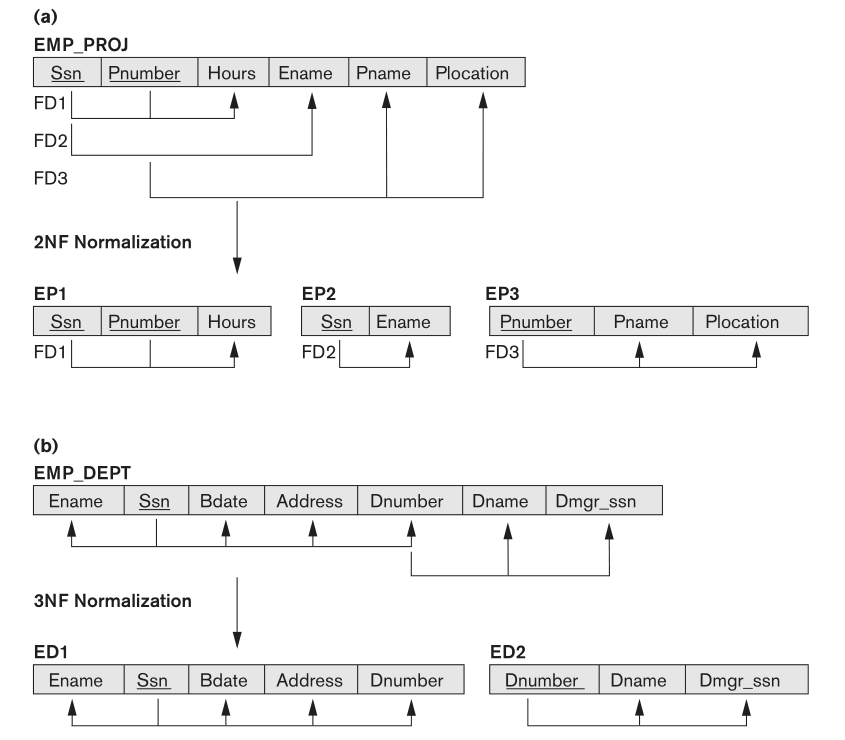
\includegraphics[scale = 0.7]{2NF.png}
\bigbreak

\subsection{Third Normal Form}

\begin{itemize}
	\item \tf{Third Normal Form (3NF) is based on the concept of \ti{transitive dependency}}.
	\item A relation schema R is in 3NF if it satisfies 2NF and no nonprime attribute of R is transitive dependent on the primary key.
\end{itemize}

\bigbreak
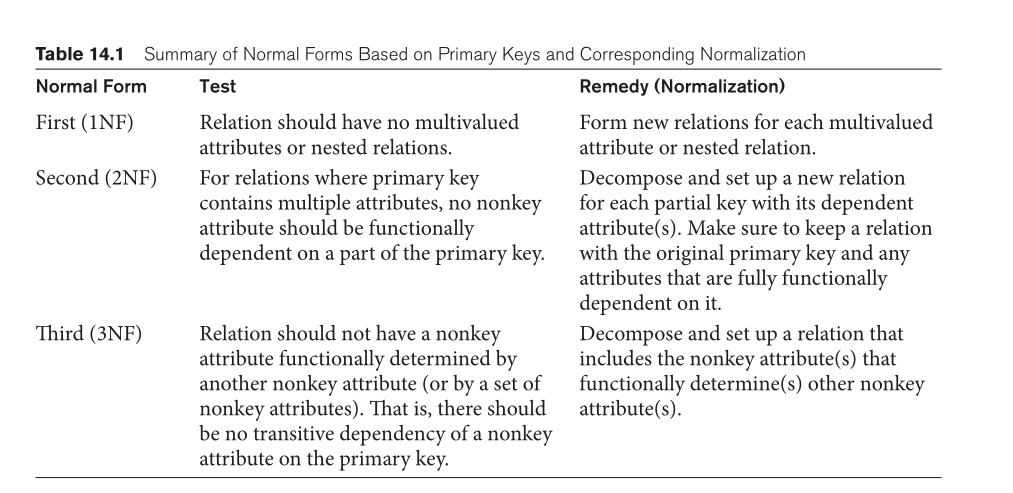
\includegraphics[scale = 0.7]{summary.png}
\bigbreak

\subsection{Boyce-Codd Normal Form}

\begin{itemize}
	\item \tf{Boyce-Codd normal form (BCNF)} was proposed as a simpler form of 3NF, but it is found to be stricter than 3NF.
	\item Every relation in BCNF is also in 3NF, a relation in 3NF is \tf{not neccessarily} in BCNF.
	\item A relation schema R is in BCNF if whenever a \ti{nontrivial} functional dependency $X \rarrow A$ holds in R, then X is a superkey of R.
\end{itemize}

\newpage
\section{Chapter 16: Disk Storage, Basic File Structures, Hashing, and Modern Storage Architectures}

\subsection{Introduction}

\begin{enumerate}
	\item \tf{Primary storage}
	\begin{itemize}
		\item This category includes storage media that can be operated on directly by the computer's central processing unit (CPU), such as the computer's main memory and smaller but faster cache memories.
		\item Provide fast access to data but is of limited storage capacity.
		\item Main memory: RAM
	\end{itemize}

	\item \tf{Secondary storage}
	\begin{itemize}
		\item SSD and HDD
	\end{itemize}

	\item \tf{Teritiary storage}
	\begin{itemize}
		\item Optical disks (CD-ROMs, DVDs, and other similar storage media) and tapes.
		\item Larger capacity, cost less, and provide slower access to data.
	\end{itemize}
\end{enumerate}

\subsubsection{Memory Hierarchies and Storage Devices}

\begin{enumerate}
	\item At the \ti{primary storage level}
	
	\begin{itemize}
		\item The memory hierarchy includes at most expensive end \tf{cache memory}, which is static RAM.
		\item  Cache memory is typically used by the CPU to speed up execution of program instructions using techniques such as prefetching and pipelining.
		\item The next level of primary storage is DRAM (dynamic RAM), which provides the main work area for the CPU for keeping program instructions and data. It is popularly called \tf{main memory}.
		\item The advantage of DRAM is its low cost, which continues to decrease; The drawback is its volatility 2 and lower speed compared with static RAM.
	\end{itemize}
	
	\item At the secondary and tertiary storage level:
	
	\begin{itemize}
		\item The hierarchy includes magnetic disks; \tf{mass storage} in the form of CD-ROM (compact disk–read-only memory) and
		DVD (digital video disk or digital versatile disk) devices; and finally tapes at the least expensive end of the hierarchy.
		\item The storage capacity is measured in terabytes (1,000 GB) and petabyte (1,000 terabytes).
		\item Generally, large permanent databases reside on secondary storage (magnetic disks), and portions of the database are brought into main memory as needed. 
		\item In some cases, entire databases can be kept in main memory (with a backup copy on magnetic disk), which results in \tf{main memory databases} $\rarrow$ useful in real-time applications that require fast response times. 
	\end{itemize}
\end{enumerate}

\tf{Flash Memory}

\begin{itemize}
	\item Flash memories are high-density, high-performance memories using EEPROM (electrically erasable programmable read-only memory) technology. 
	\item Advantage: fast access speed.
	\item Disadvantage: an entire block must be erased and written over simultaneously. 
	\item Flash memories come in two types called NAND and NOR flash based on the type of logic circuits used. The NAND flash devices have a higher storage capacity for a given cost. 
	\item Flash devices are used in cameras, MP3/MP4 players, cell phones, PDAs (personal digital assistants), USB (universal serial bus) flash drives or USB sticks and so on.
\end{itemize}

\tf{Optical Drives}
\begin{itemize}
	\item CDs have a 700-MB capacity whereas DVDs have capacities ranging from 4.5 to 15 GB. 
	\item CD-ROM (compact disk – read only memory) disks store data optically and are read by a laser. CD-ROMs contain prerecorded data that cannot be overwritten.
	\item CD-R (compact disk recordable) and DVD-R or DVD+R, also known as WORM (write-once-read-many) disks, allow data to be written once and read any number of times without the possibility of erasing. They hold about half a gigabyte of data per disk and last much longer than magnetic disks. 
	\item A higher capacity format for DVDs called Blu-ray DVD can store 27 GB per layer, or 54 GB in a two-layer disk.  
	\item \tf{Optical jukebox memories} use an array of CD-ROM platters, which are loaded onto drives on demand. Their retrieval times are in the hundreds of milliseconds, quite a bit slower than magnetic disks. 
\end{itemize}

\tf{Magnetic Tapes:} \tf{Tape jukeboxes} — which contain a bank of tapes that are catalogued and can be automatically loaded onto tape drives—are becoming popular as \tf{tertiary storage} to hold terabytes of data. 

\bigbreak
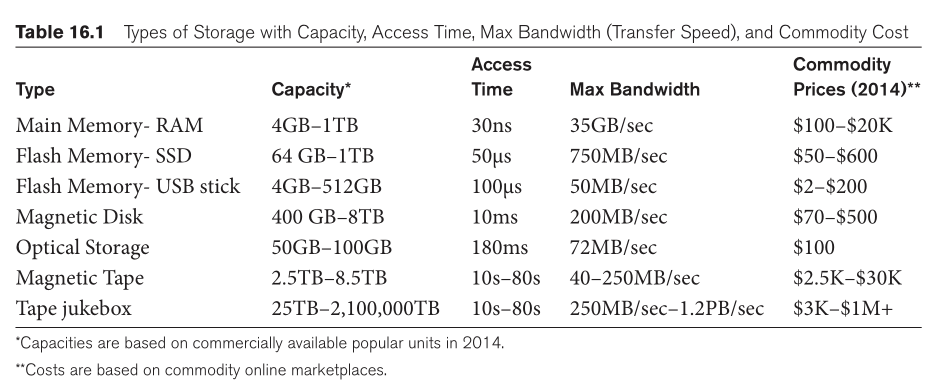
\includegraphics[scale = 0.7]{typeStorage.png}
\bigbreak

\subsubsection{Storage Organization of Databases}

\begin{itemize}
	\item Databases store large amounts of data that must persist over long periods of time, and hence the data is often referred to as \tf{persistent data}. 
	\item {Transient data}, which are accessed and processed repeatedly, persists for only a limited time.
	\item Most databases are stored permanently (or persistently) on magnetic disk secondary storage, for the following reasons: 
	\begin{itemize}
		\item Databases are too large to fit entirely in main memory.
		\item The circumstances that cause permanent loss of stored data arise less frequently for disk secondary storage than for primary storage; Secondary storage is \tf{nonvolatile}.
		\item The cost of storage per unit of data is an order of magnitude less for disk secondary storage than for primary storage. 
	\end{itemize}

	\item Magnetic tapes are frequently used for backing up databases because they cost much less. 
	\item Tapes or optical removable disks must be loaded and read before the data becomes available for processing. In contrast, disks are online devices that can be accessed directly at any time. 
	\item The data stored on disk is organized as \tf{files of records}. 
	\item Each record is a collection of data values that can be interpreted as facts about entities, their attributes, and their relationships.
\end{itemize}

\subsection{Secondary Storage Devices}

\subsubsection{Hardware Description of Disk Devices}

\begin{itemize}
	\item All disks are made of magnetic material shaped as a thin circular disk, and protected by a plastic or acrylic cover. (a)
	\item A disk is \tf{single-sided} if it stores information on one of its surfaces only and {double- sided} if both surfaces are used. 
	\item To increase storage capacity, disks are assembled into a \tf{disk pack}, which may include many disks and therefore many surfaces. (b)
	
	\bigbreak
	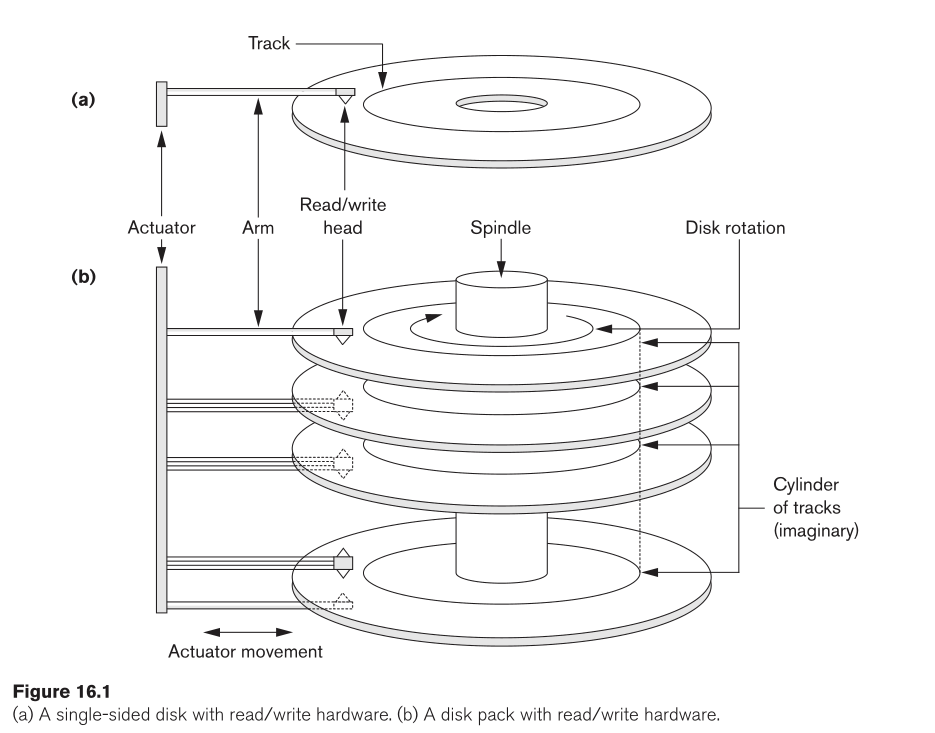
\includegraphics[scale = 0.7]{disk.png}
	\bigbreak

	\item The two most common form factors are 3.5 and 2.5-inch diameter. 
	\item Information is stored on a disk surface in concentric circles of small width, each having a distinct diameter.
	\item Each cycle is called \tf{track}, tracks with the same diameter on the various surfaces are called a \tf{cylinder} because of the shape they would form if connected in space.
	\item Data stored on one cylinder can be retrieved much faster than if it were distributed among different cylinders. 
	\item The number of tracks on a disk ranges from a few thousand to 152,000, and the capacity of each track typically ranges from tens of kilobytes to 150 KBs.
	\item Because a track usually contains a large amount of information, it is divided into smaller arcs or sectors. The division of a track into sectors is hard-coded on the disk surface and cannot be changed.
	
	\bigbreak
	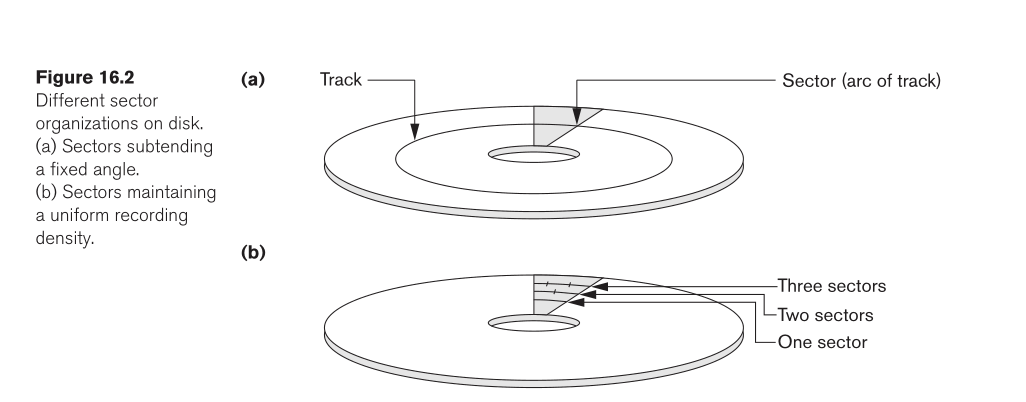
\includegraphics[scale = 0.7]{sector.png}
	\bigbreak

	\item The division of a track into equal-sized \tf{disk blocks} (or \tf{pages - track sectors}) is set by the operating system during disk \tf{formatting} (or \tf{initialization}).
	\item Block size (ranging from 512 to 8192 bytes) is fixed during initialization and cannot be changed dynamically.
	\item A disk with hard-coded sectors often has the sectors subdivided or combined into blocks during initialization. 
	\item Blocks are separated by fixed-size \tf{interblock gaps}, which include coded information written during disk initialization used to determine which block on the track follows each interblock gap. 
	\item A disk is a random access addressable device. 
	\item Transfer of data between main memory and disk takes place in units of disk blocks. 
	\item The \tf{hardware address} of a block — a combination of a cylinder number, track number and block number — is supplied to the disk I/O hardware. In modern disk drives, a single number called LBA (logical block address), which is a number between 0 and n, is mapped automatically to the right block by the disk drive controller. 
	\item The address of a \tf{buffer} — a contiguous reserved area in main storage that holds one disk block—is also provided.
	\item  For a \tf{read} command, the disk block is copied into the buffer; for a \tf{write} command, the contents of the buffer are copied into the disk block. 
	\item Sometimes several contiguous blocks, called a \tf{cluster}, may be transferred as a unit. 
	\item The actual hardware mechanism that reads or writes a block is the disk read/write head.
	\item A disk or disk pack is mounted in the disk drive, which includes a motor that rotates the disks. 
	\item A read/write head includes an electronic component attached to a \tf{mechanical arm}. Disk packs with multiple surfaces are controlled by several read/write heads—one for each surface.
	\item All arms are connected to an actuator attached to another electrical motor, which moves the read/write heads and positions them precisely over the cylinder of tracks specified in a block address. 
	\item The disk pack rotates continuously at a constant speed (between 5,400 and 15,000 rpm). 
	\item The disk pack rotates continuously at a constant speed (between 5,400 and 15,000 rpm). 
	\item Some disk units have fixed read/write heads, with as many heads as there are tracks. These are called \tf{fixed-head disks}, whereas disk units with an actuator are called \tf{movable-head disks}.
	\item For fixed-head disks, a track or cylinder is selected by switching to the appropriate read/write head rather than by actual mechanical movement; consequently, it is much faster. However, the cost of the additional read/write heads is high. 
\end{itemize}

\tf{Interfacing Disk Drives to Computer Systems}

\begin{itemize}
	\item A \tf{disk controller}, typically embedded in the disk drive, controls the disk drive and interfaces it to the computer
	system.
	\item SCSI: small computer system interface.
	\item SATA: Serial AT Attachment, also known as NL-SAS (Nearline SAS).
	\item SAS: Serial Attached SCSI.
	\item \tf{Seek time:} the time required to mechanically position the read/write head on the correct track (5 to 10 msec on desktops and 3 to 8 msec on servers)
\end{itemize}

\subsubsection{Making Data Access More Efficient on Disk}

\begin{enumerate}
	\item Buffering of Data.
	\item Proper organization of data on disk.
	\item Reading data ahead of request.
	\item Proper scheduling of I/O requests.
	\item Use of log disks to temporarily hold writes.
	\item Use of SSDs or flash memory for recovery purposes.
\end{enumerate}

\subsubsection{SolidState Device (SSD) Storage}

\begin{itemize}
	\item The recent trend is to use flash memories as an intermediate layer between main memory and secondary storage.
	\item The main component of an SSD is a controller and a set of interconnected flash memory cards. Use of NAND flash memory is most common. 
	\item Typically, when a write to disk occurs on an HDD, the same block is overwritten with new data. In SSDs, the data is written to different NAND cells to attain \tf{wear-leveling}, which prolongs the life of the SSD.
	\item DRAM-based SSDs are also available. They are costlier than flash memory, but they offer faster access times of around 10 micro s as opposed to 100 micro s for flash. Their main drawback is that they need an internal battery or an adapter to supply power. 
\end{itemize}

\subsubsection{Magnetic Tape Storage Devices}

\begin{itemize}
	\item Not supporting \tf{random access} like disks, Magnetic tapes are sequential access devices; to access the nth block on tape, first we must scan the preceding n – 1 blocks.
	\item Data is stored on reels of high-capacity magnetic tape, somewhat similar to audiotapes or videotapes. A tape drive is required to read the data from or write the data to a tape reel. 
	\item A read/write head is used to read or write data on tape. Data records on tape are also stored in blocks larger than those for disks and interblock gaps are also quite large. 
	\item Magnetic Tape is best used for:
	\begin{itemize}
		\item Backing up data storage.
		\item Store excessively large database files that are outdated but required for historical recordkeeping. 
	\end{itemize}

	\item Originally, half-inch reel tape drives used nine-track tapes for data storage. Later, smaller 8-mm magnetic tapes that can store up to 50 GB become a popular backup media.
\end{itemize}

\subsection{Placing File Records on Disk}

\subsubsection{Records and Record Types}

\begin{itemize}
	\item An entity type can be referred to as a \tf{record type} or \tf{record format}. 
	\item The instances of an entity type can be referred to as \tf{records}.
	\item Each record can have one or more \tf{fields} (attributes) with their own \tf{data type}: numeric (integer, long integer, or floating point), string of characters (fixed-length or varying), Boolean (having 0 and 1 or TRUE and FALSE values only), and sometimes specially coded \tf{date} and \tf{time} data types. 
\end{itemize}

\subsubsection{Files, Fixed-Length Records, and Variable-Length Records}

\begin{itemize}
	\item A file is a sequence of records. 
	\item If every record in the file has exactly the same size (in bytes), the file is said to be made up of \tf{fixed-length records}. 
	\item If different records in the file have different sizes, the file is said to be made up of \tf{variable-length records}.
	\item A file may have variable-length records for several reasons: 
	\begin{itemize}
		\item The file records are of the same record type, but one or more of the fields are of varying size (\tf{variable-length fields}).
		\item The file records are of the same record type, but one or more of the fields may have multiple values for individual records; such a field is called a \tf{repeating field} and a group of values for the field is called a \tf{repeating group}.
		\item The file records are of the same record type, but one or more of the fields are \tf{optional}.
		\item The file contains records of \ti{different record types} and hence of varying size (\tf{mixed file}). This would occur if related records of different types were \ti{clustered} (placed together) on disk blocks.  
	\end{itemize}
\end{itemize}

\subsubsection{Allocating File Blocks on Disk}

\begin{itemize}
	\item \tf{Contiguous Allocation:} the file blocks are allocated to consecutive disk blocks $\rarrow$ Fast reading using double buffering but difficult to expand the file.
	\item \tf{Linked Allocation:} Each file block contains a pointer to the next file block $rarrow$ Easy to expend the file but slow to read it. 
	\item A combination of the two techniques above allocates \tf{clusters} of consecutive disk blocks, and the clusters are linked. Clusters are sometimes called \tf{file segments} or \tf{extents}
	\item \tf{Indexed allocation}: where one or more \tf{index blocks} contain pointers to the actual file blocks.  
\end{itemize}

\section{Chapter 17: Indexing Structures for Files}

\end{document}






